\section{Storage}

$Revision: 1.19 $

Figure \ref{fig:storage}
presents basic \api{Storage} modules and their API.

\begin{figure}
	\centering
	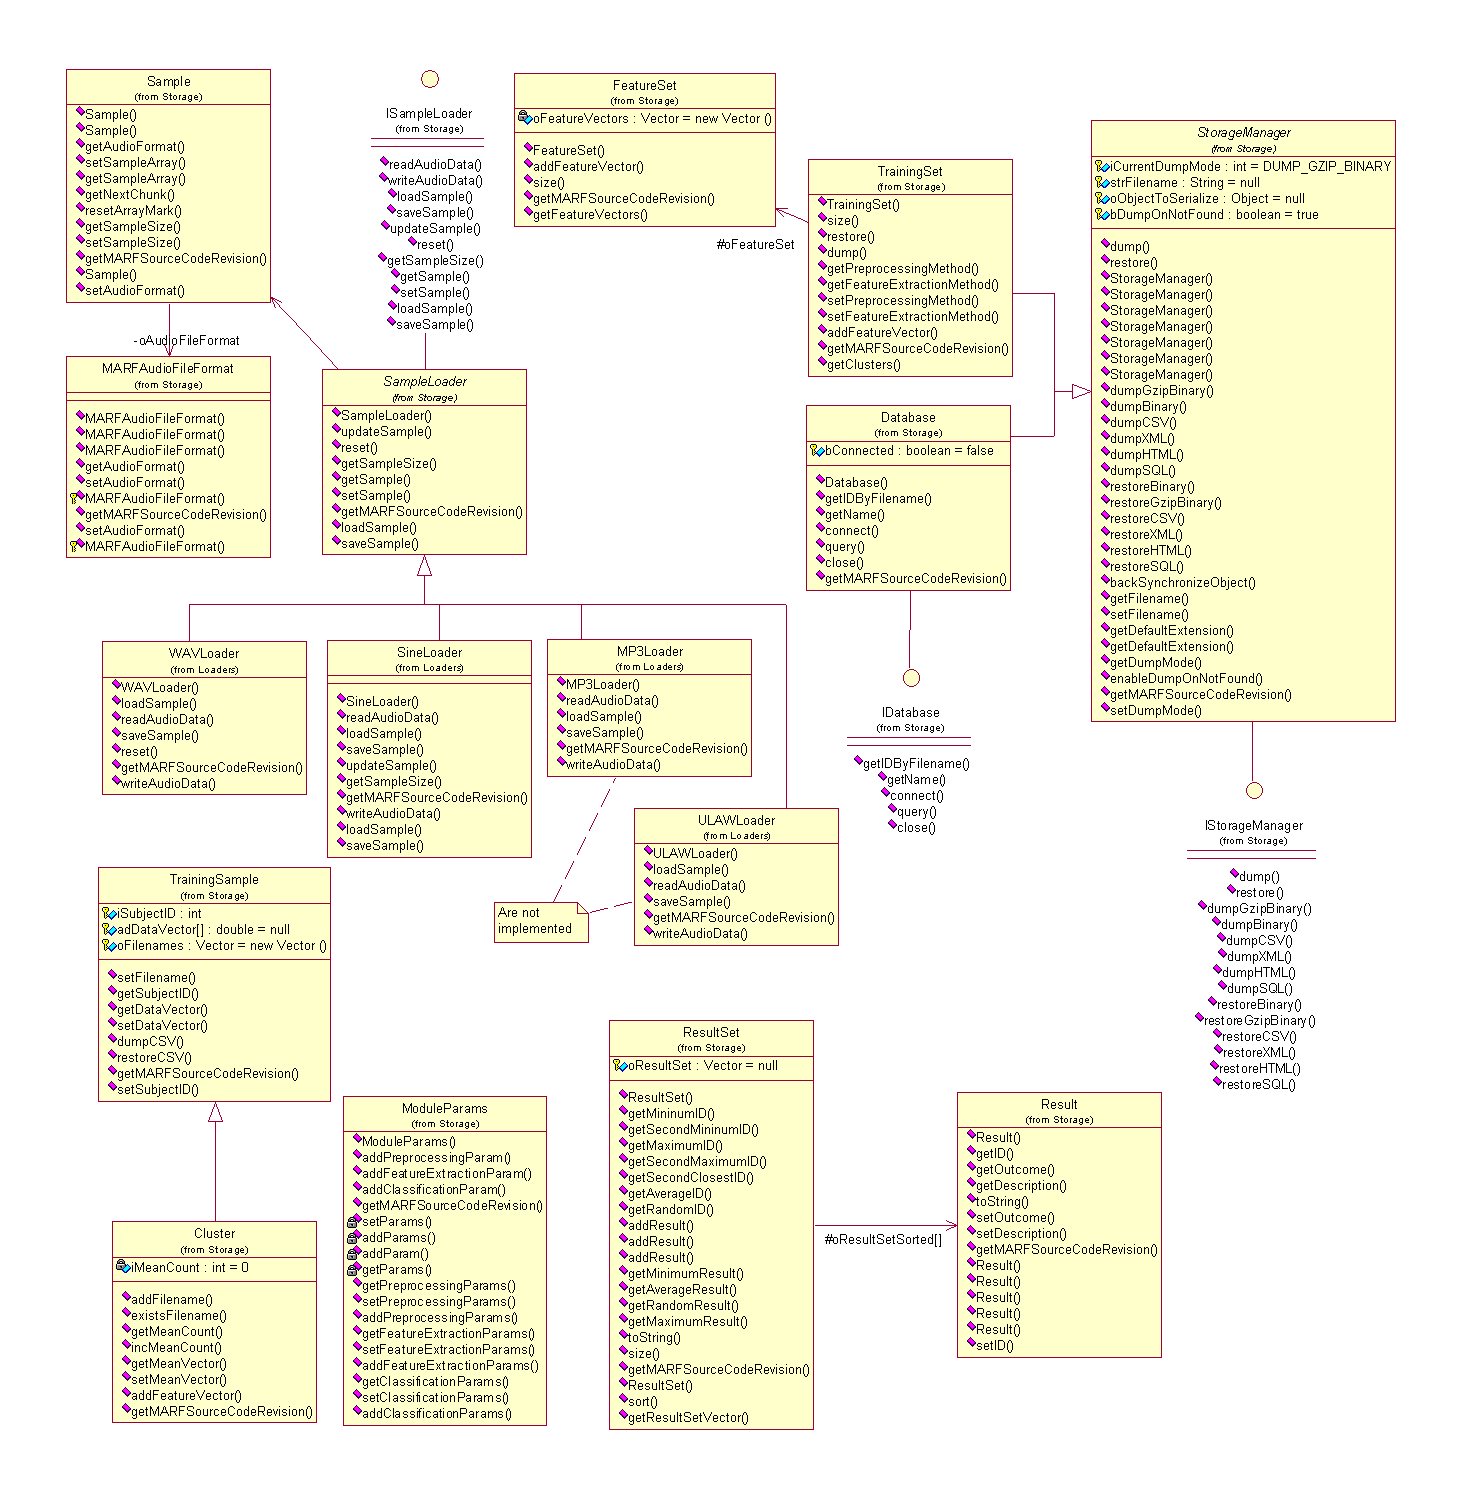
\includegraphics[angle=90,totalheight=660pt,width=550pt]{../graphics/arch/storage.png}
	\caption{Storage}
	\label{fig:storage}
\end{figure}

\subsection{Speaker Database}

We store specific speakers in a comma-separated (CSV) file, \verb+speakers.txt+
within the application.
It has the following format:

\verb+<id:int>,<name:string>,<training-samples:list>,<testing-samples:list>+

Sample lists are defined as follows:

\verb+<*-sample-list> := filename1.wav|filename2.wav|...+


\subsection{Storing Features, Training, and Classification Data}

We defined a standard \verb+StorageManager+ interface for the modules to use.
That's part of the \verb+StorageManager+ interface which each module will override
because each a module has to know how to serialize itself, but the applications
using {\marf} should not care.
Thus, this \verb+StorageManager+ is a base class with abstract methods \verb+dump()+ and
\verb+restore()+. These methods would generalize the
model's serialization, in the sense that they are somehow ``read'' and ``written''.

We have to store data we used for training for later use in
the classification process. For this we pass FFT (\xf{sect:fft}) and LPC (\xf{sect:lpc})
feature vectors through the \verb+TrainingSet+/\verb+TrainingSample+ class pair,
which, as a result, store mean vectors (clusters) for our training models.

In the Neural Network we use XML. The only reason XML and text files
have been suggested is to allow us to easily modify values in
a text editor and verify the data visually.

In the Neural Network classification, we are using one net for
all the speakers. We had thought that one net for each speaker
would be ideal, but then we'll lose too much discrimination
power. But doing this means that the net will need complete
re-training for each new training utterance (or group thereof).

We have a training/testing script that lists the location of all the wave files to
be trained along with the identification of the speaker - \verb+testing.sh+.

%All resulting vectors (and associated speakers) are appended to the \verb+training.set+ file.
%Then the model is re-trained on whatever data needed and new models are dumped.

%In the stochastic models, if we had them, the complete set of
%utterances will be needed for the speaker to which the new
%utterance(s) are being added, for mean and variance calculations. This
%implies that all data needs storing.

\subsection{Assorted Training Notes}

$Revision: 1.6 $

For training we are using sets of feature vectors created by \api{FFT} or
\api{LPC} and passing them to the \api{NeuralNetwork} in the form of a 
cluster, or rather probabilistic ``cluster''. With this, there are some
issues:

\begin{enumerate}
\item
Mapping. We have to have a record of speakers and IDs for these speakers.
This can be the same for \api{NeuralNetwork} and \api{Stochastic} methods so long as the \api{NeuralNetwork}
will return the proper number and the ``clusters'' in the \api{Stochastic} module have
proper labeling.

\item
Feature vector generation. I think the best way to do this is for each
application using {\marf} to specify a feature file or directory which will
contain lines/files with the following info:

\verb+[a1, a2, ... , an] : <speaker id>+

Retraining for a new speaker would involve two phases 1) appending the
features to the file/dir, then 2) re-training the models. The
\api{Classification} modules will be aware of the scheme and re-train on all data
required.
\end{enumerate}

\subsubsection{Clusters Defined}

Given a set of feature vectors in $n$-dimensional space, if we want these to
represent $m$ ``items'' (in our case, speakers), we can make groupings of
these vectors with a center point $c_{i}$ (ie: $m$ center points which will
then represent the ``items''). Suen discussed an iterative algorithm to find
the optimal groupings (or clusters).
Anyway, I don't believe that Suen's clustering stuff is at all useful, as
we will know, through info from training, which speaker is associated with
the feature vector and can create the ``clusters'' with that information.

So for \api{NeuralNetwork}: no clusters, just regular training.
So for \api{Stochastic}: Clusters (kind of). I believe that we need to represent
a Gaussian curve with a mean vector and a co-variance matrix. This will be
created from the set of feature vectors for the speaker. But again, we know
who it is so the Optimal Clustering business is useless.

% EOF


\subsection{File Location}

We decided to keep all the data and intermediate files in the same
directory or subdirectories of that of the application.

\begin{itemize}

\item \verb+marf.Storage.TrainingSet.*+ - represent training sets
	(global clusters) used in training with different preprocessing and feature extraction
	methods; they can either be gzipped binary (.bin) or CSV text (.csv).

\item \verb+speakers.txt.stats+ - binary statistics file.

\item \verb+marf.Classification.NeuralNetwork.*.xml+ - XML file representing a trained
	Neural Net for all the speakers in the database.

\item \verb+training-samples/+ - directory with WAV files for training.

\item \verb+testing-samples/+ - directory with WAV files for testing.

\end{itemize}

\subsection{Sample and Feature Sizes}

Wave files are read and outputted as an array of
data points that represents the waveform of the signal.

Different methods will have different feature vector sizes.
It depends on what kind of precision one desires.
In the case of FFT, a 1024 FFT will result in 512 features,
being an array of ``doubles'' corresponding to the frequency range.

\cite{shaughnessy2000} said about using 3 ms for phoneme analysis and
something like one second for general voice analysis.  At 8 kHz, 1024 samples
represents 128 ms, this might be a good compromise.

\subsection{Parameter Passing}

A generic \verb+ModuleParams+ container class has been created to for an application
to be able to pass module-specific parameters when
specifying model files, training data,
amount of LPC coefficients, FFT window size, logging/stats files, etc.

\subsection{Result}

When classification is over, its result should be stored somehow
for further retrieval by the application. We have defined
the \verb+Result+ object to carry out this task. It contains
ID of the subject identified as well as some additional statistics
(such as second closest speaker and distances from other speakers, etc.)

\subsection{Sample Format}

$Revision: 1.20 $

The sample format used for our samples was the following:

\begin{itemize}
	\item Audio Format: PCM signed (WAV)
	\item Sample Rate: 8000 Hz
	\item Audio Sample Size: 16 bit
	\item Channels: 1 (mono)
	\item Duration: from about 7 to 20 seconds
\end{itemize}

All training and testing samples were recorded through an external sound recording
program (MS Sound Recorder) using a standard microphone. Each sample was
saved as a WAV file with the above properties and stored in the appropriate folders
where they would be loaded from within the main application. The PCM audio format
(which stands for Pulse Code Modulation) refers to the digital encoding of the audio
sample contained in the file and is the format used for WAV files. In a PCM
encoding, an analog signal is represented as a sequence of amplitude values. The
range of the amplitude value is given by the audio sample size which represents the
number of bits that a PCM value consists of. In our case, the audio sample size is
16-bit which means that that a PCM value can range from 0 to 65536. Since we are
using PCM-signed format, this gives an amplitude range between $-32768$ and $32768$.
That is, the amplitude values of each recorded sample can vary within this range.
Also, this sample size gives a greater range and thus provides better accuracy in
representing an audio signal then using a sample size of 8-bit which limited to a
range of $(-128, 128)$. Therefore, a 16-bit audio sample size was used for our
experiments in order to provide the best possible results. The sampling rate refers
to the number of amplitude values taken per second during audio digitization.
According to the Nyquist theorem, this rate must be at least twice the maximum rate
(frequency) of the analog signal that we wish to digitize (\cite{jervis}). Otherwise, the signal
cannot be properly regenerated in digitized form. Since we are using an 8 kHz
sampling rate, this means that actual analog frequency of each sample is limited to
4 kHz. However, this limitation does not pose a hindrance since the difference in
sound quality is negligible (\cite{shaughnessy2000}). The number of channels
refers to the output of the sound (1 for mono and 2 for stereo -- left and right
speakers). For our experiment, a single channel format was used to avoid complexity
during the sample loading process.

\subsection{Sample Loading Process}

To read audio information from a saved voice sample, a special sample-loading
component had to be implemented in order to load a sample into an internal data
structure for further processing. For this, certain sound libraries (\verb+javax.sound.sampled+)
were provided from the Java programming language which enabled us to
stream the audio data from the sample file. However once the data was captured, it
had to be converted into readable amplitude values since the library routines only
provide PCM values of the sample. This required the need to implement special
routines to convert raw PCM values to actual amplitude values (see \verb+SampleLoader+ class in
the \verb+Storage+ package).

\clearpage
The following pseudo-code represents the algorithm used to convert the PCM values
into real amplitude values (\cite{javasun}):

\vspace{15pt}
\hrule
\begin{verbatim}
function readAmplitudeValues(Double Array : audioData)
{
    Integer: MSB, LSB,
             index = 0;

    Byte Array: AudioBuffer[audioData.length * 2];

    read audio data from Audio stream into AudioBuffer;

    while(not reached the end of stream OR index not equal to audioData.length)
    {
        if(Audio data representation is BigEndian)
        {
            // First byte is MSB (high order)
            MSB = audioBuffer[2 * index];
            // Second byte is LSB (low order)
            LSB = audioBuffer[2 * index + 1];
        }
        else
        {
            // Vice-versa...
            LSB = audioBuffer[2 * index];
            MSB = audioBuffer[2 * index + 1];
        }

        // Merge high-order and low-order byte to form a 16-bit double value.
        // Values are divided by maximum range
        audioData[index] = (merge of MSB and LSB) / 32768;
    }
}
\end{verbatim}
\hrule
\vspace{15pt}

This function reads PCM values from a sample stream into a byte array that has
twice the length of \verb+audioData+; the array which will hold the converted amplitude
values (since sample size is 16-bit). Once the PCM values are read into \verb+audioBuffer+,
the high and low order bytes that make up the amplitude value are extracted
according to the type of representation defined in the sample's audio format.
If the data representation is {\it big endian}, the high order byte of each PCM value is
located at every even-numbered position in \verb+audioBuffer+. That is, the high order
byte of the first PCM value is found at position 0, 2 for the second value, 4 for
the third and so forth. Similarly, the low order byte of each PCM value is located
at every odd-numbered position (1, 3, 5, etc.). In other words, if the data
representation is {\it big endian}, the bytes of each PCM code are read from left to
right in the \verb+audioBuffer+. If the data representation is not {\it big endian}, then high
and low order bytes are inversed. That is, the high order byte for the first PCM
value in the array will be at position 1 and the low order byte will be at
position 0 (read right to left). Once the high and low order bytes are properly
extracted, the two bytes can be merged to form a 16-bit double value. This value is
then scaled down (divide by 32768) to represent an amplitude within a unit range $(-1, 1)$.
The resulting value is stored into the \verb+audioData+ array, which will be passed to
the calling routine once all the available audio data is entered into the array. An
additional routine was also required to write audio data from an array into wave
file. This routine involved the inverse of reading audio data from a sample file
stream. More specifically, the amplitude values inside an array are converted back
to PCM codes and are stored inside an array of bytes (used to create new audio
stream). The following illustrates how this works:

\vspace{15pt}
\hrule
\begin{verbatim}
public void writePCMValues(Double Array: audioData)
{
    Integer: word  = 0,
             index = 0;

    Byte Array: audioBytes[(number of ampl. values in audioData) * 2];

    while(index not equal to (number of ampl. values in audioData * 2))
    {
        word = (audioData[index] * 32768);
        extract high order byte and place it in appropriate position in audioBytes;
        extract low order byte and place it in appropriate position in audioBytes;
    }

    create new audio stream from audioBytes;
}
\end{verbatim}
\hrule
\vspace{15pt}

% EOF


\section{Assorted File Format Notes}

$Revision: 1.4 $


	We decided to stick to Mono-8000Hz-16bit WAV files.  8-bit might be
	okay too, but we could retain more precision with 16-bit files.  8000Hz is
	supposed to be all you need to contain all frequencies of the vocal
	spectrum
	(according to Nyquist anyways...).  If we use 44.1 kHz we'll just be wasting
	space and computation time.

	There are also MP3 and ULAW and other file format loaders stubs which are unimplemented
	as of this version of MARF.

Also: I was just thinking I think I may have made a bit of a mistake
downsampling to 8000Hz... I was saying that the voice ranges to about 8000Hz so
that's all we should need for the samples, but then I realized that if you have
an 8000Hz sample, it actually only represents 4000Hz, which would account for
the difference I noticed.. but maybe we should be using 16KHz samples.  On the
other hand, even at 4KHz the voice is still perfectly distinguishable...


I tried the WaveLoader with one of the samples provided by Stephen
(jimmy1.wav naturally!) and got some nice results! I graphed the PCM
obtained from the getaudioData() function and noticed quite a difference
from the PCM graph obtained with my ``test.wav". With ``test.wav", I was
getting unexpected results as the graph (``rawpcm.xls") didn't resemble any
wave form. This lead me to believe that I needed to convert the data on
order to represent it in wave form (done in the ``getWaveform()" function).
But after having tested the routine with ``jimmy1.wav", I got a beautiful
wave-like graph with just the PCM data which makes more sense since PCM
represents amplitude values! The reason for this is that my ``test.wav"
sample was actually 8-bit mono (less info.) rather than 16-bit mono as with
Stephen's samples. So basically, we don't need to do any ``conversion" if we
use 16-bit mono samples and we can scrap the ``getWaveform()" function.
I will come up with a ``Wave" class sometime this week which will take care
of loading wave files and windowing audio data. Also, we should only read
audio data that has actual sound, meaning that any silence (say -10 < db <
10) should be discarded from the sample when extracting audio data.
Just thinking out loud!

I agree here.  I was thinking perhaps the threshold could be determined from
the ``silence" sample.

% EOF


% EOF
